\section{Fichas técnicas}
\label{anexo:ficha tecnica}

\subsection{Ficha técnica KYMCO Agility Carry 50 E5}
\label{subanexo: ficha tecnica kymco 50}

\begin{figure}[H]
    \centering
    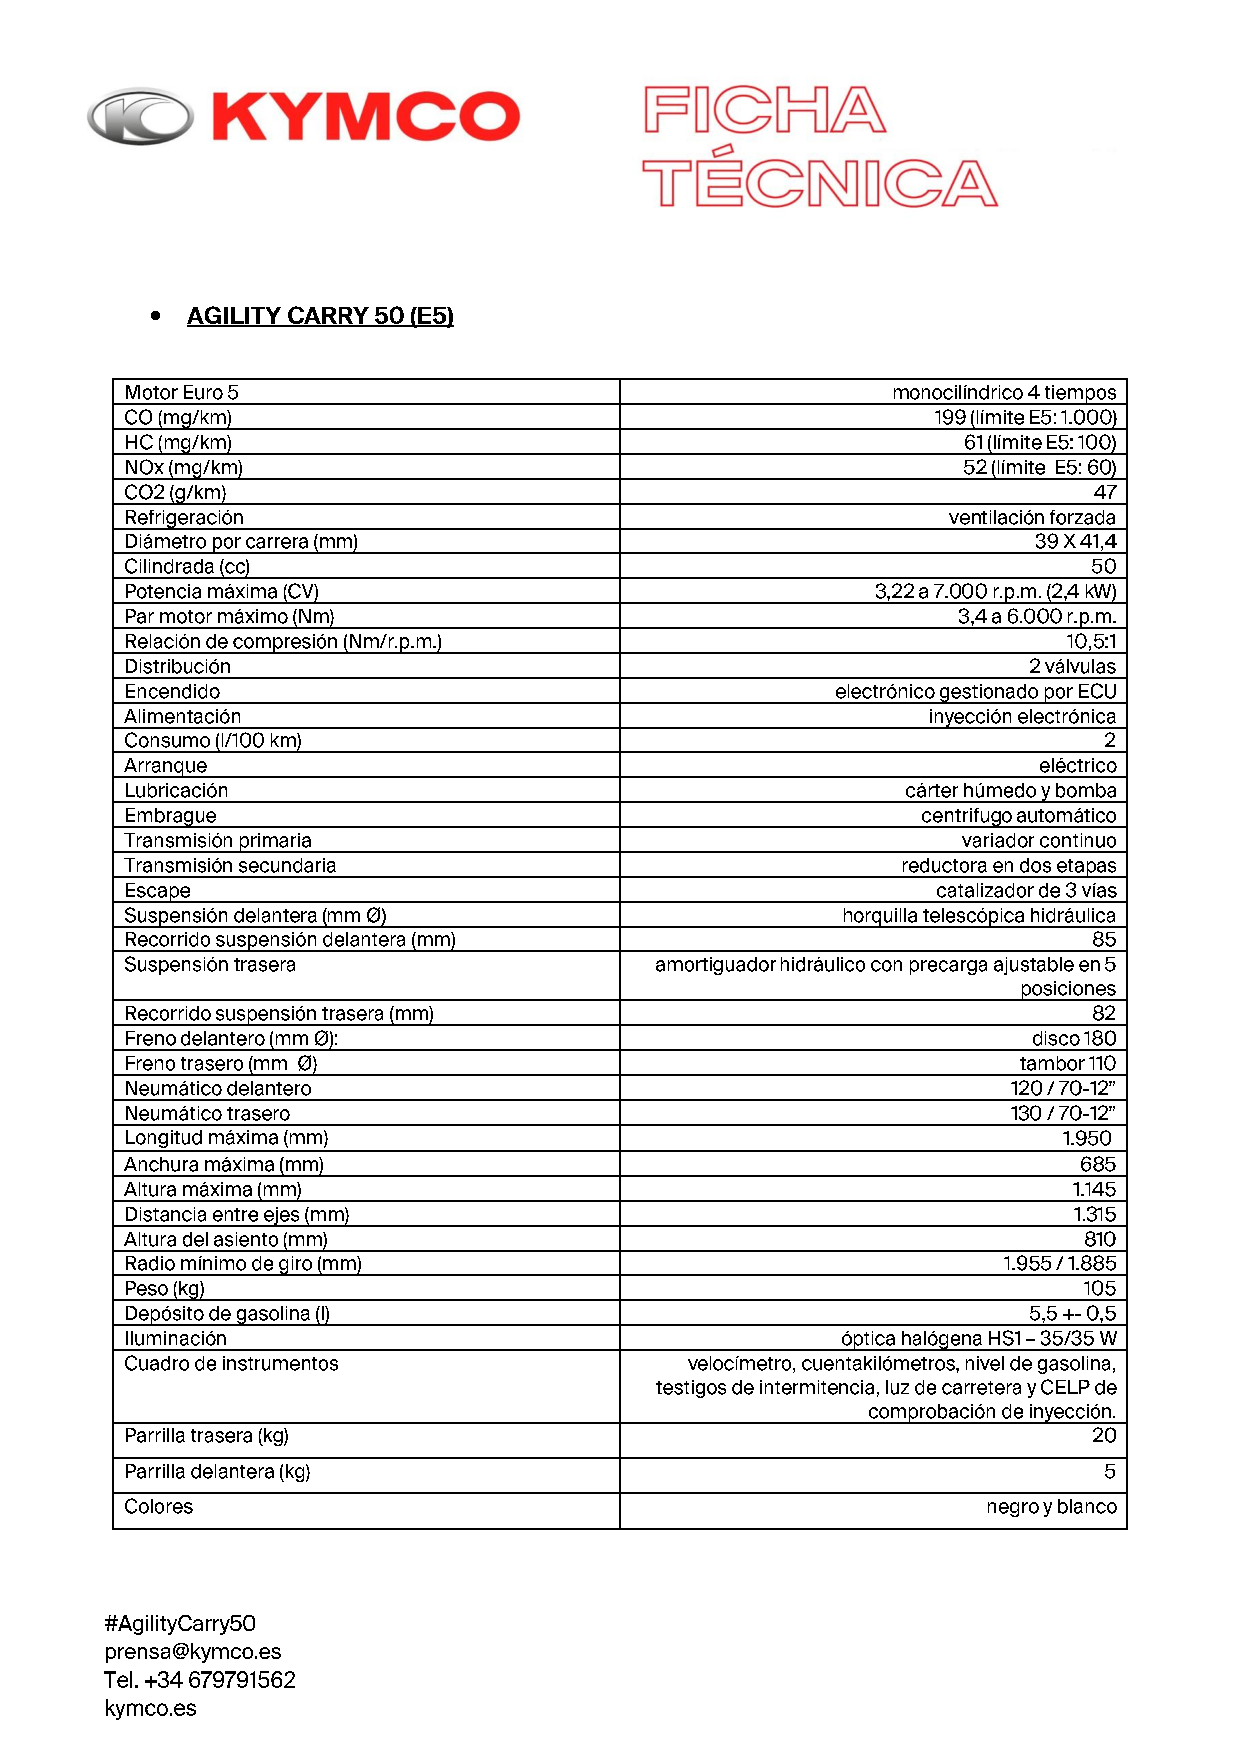
\includegraphics[scale = 0.7]{archivos/ficha_tecnica_motillo_peter.pdf}
    \caption{Ficha Técnica KYMCO Agility Carry 50 E5.}
    \label{fig: ficha tecnica KYMCO 50}
\end{figure}

%Jorge, encuentrame

\subsection{Ficha técnica KYMCO Agility Carry 125}
\label{subanexo: ficha tecnica kymco 125}

\begin{table}[H]
\centering
\begin{tabular}{l}
\multicolumn{1}{c}{\textbf{Datos comerciales KYMCO Agility Carry 125 2021-2022}} \\ \hline
\textbf{Marca:}                  \\
KYMCO                            \\
\textbf{Tipo de carnet:}         \\
125cc                            \\
\textbf{Año:}                    \\
2021                             \\
\textbf{Plazas:}                 \\
1                                \\
                                 \\
\multicolumn{1}{c}{\textbf{Motor y transmisión}}                                 \\ \hline
\textbf{Cilindrada exacta:}      \\
125 cc                           \\
\textbf{Tipo:}                   \\
4 T                              \\
\textbf{Distribución:}           \\
SOHC                             \\
\textbf{Cilindros:}              \\
1                                \\
\textbf{Válvulas por cilindro:}  \\
2                                \\
\textbf{Alimentación:}           \\
Inyección electrónica            \\
\textbf{Refrigeración:}          \\
Aire forzado                     \\
\textbf{Diámetro por carrera:}   \\
52.4 mm x 57.8 mm                \\
\textbf{Compresión:}             \\
9.6 :1                           \\
\textbf{Potencia máxima declarada:}                                              \\
9.12 CV a 7.500 rpm              \\
\textbf{Combustible:}            \\
Gasolina sin plomo 95            \\
\textbf{Normativa anticontaminación:}                                            \\
Euro5                            \\
\textbf{Encendido:}              \\
Electrónico CDI                  \\
\textbf{Transmisión secundaria:} \\
Correa                           \\
\textbf{Embrague:}               \\
Automático centrífugo en seco   
\end{tabular}
\end{table}

\begin{table}[H]
\centering
\begin{tabular}{lll}
\multicolumn{1}{c}{\textbf{Suspensión delantera}} &  & \multicolumn{1}{c}{\textbf{Suspensión trasera}} \\ \cline{1-1} \cline{3-3} 
\textbf{Tipo de suspensión delantera:}       &  & \textbf{Tipo basculante:}                       \\
Horquilla telescópica                        &  & Motor                                           \\
\textbf{Diámetro de barras:}                 &  & \textbf{Tipo de suspensión trasera:}            \\
31 mm                                        &  & Doble amortiguador                              \\
\textbf{Recorrido:}                          &  & \textbf{Recorrido:}                             \\
85 mm                                        &  & 82 mm                                           \\
\textbf{}                                    &  & \textbf{Regulaciones:}                          \\
\multicolumn{1}{c}{\textbf{}}                &  & Cinco puntos de precarga                        \\
\textbf{}                                    &  & \textbf{}                                       \\
\multicolumn{1}{c}{\textbf{Freno delantero}} &  & \multicolumn{1}{c}{\textbf{Freno trasero}}      \\ \cline{1-1} \cline{3-3} 
\textbf{Sistema:}                            &  & \textbf{Sistema:}                               \\
Disco (CBS)                                  &  & Disco                                           \\
\textbf{Diámetro:}                           &  & \textbf{Diámetro:}                              \\
220 mm                                       &  & 200 mm                                          \\
\textbf{Pinza:}                              &  & \textbf{}                                       \\
3 pistones                                   &  & \multicolumn{1}{c}{\textbf{}}                   \\
\textbf{}                                    &  & \textbf{}                                       \\
\multicolumn{1}{c}{\textbf{Rueda delantera}} &  & \multicolumn{1}{c}{\textbf{Rueda trasera}}      \\ \cline{1-1} \cline{3-3} 
\textbf{Diámetro de llanta:}                 &  & \textbf{Diámetro de llanta:}                    \\
12 "                                         &  & 12 "                                            \\
\textbf{Marca de neumáticos:}                &  & \textbf{Marca de neumáticos:}                   \\
CST                                          &  & CST                                             \\
\textbf{Medida de neumáticos:}               &  & \textbf{Medida de neumáticos:}                  \\
120/70-12                                    &  & 130/70-12                                       \\
\textbf{}                                    &  &                                                 \\
\textbf{}                                    &  & \textbf{}                                       \\
\multicolumn{1}{c}{\textbf{Chasis}}          &  & \multicolumn{1}{c}{\textbf{Dimensiones y peso}} \\ \cline{1-1} \cline{3-3} 
\textbf{Tipo de chasis:}                     &  & \textbf{Longitud máxima:}                       \\
Tubular                                      &  & 1.925 mm                                        \\
                                             &  & \textbf{Anchura máxima:}                        \\
\textbf{}                                    &  & 695 mm                                          \\
\textbf{}                                    &  & \textbf{Altura máxima:}                         \\
\textbf{}                                    &  & 1.100 mm                                        \\
\textbf{}                                    &  & \textbf{Distancia entre ejes:}                  \\
\textbf{}                                    &  & 1.310 mm                                        \\
\textbf{}                                    &  & \textbf{Altura de asiento:}                     \\
\textbf{}                                    &  & 790 mm                                          \\
                                             &  & \textbf{Ángulo de dirección:}                   \\
\textbf{}                                    &  & 40 º                                            \\
\textbf{}                                    &  & \textbf{Capacidad del depósito:}                \\
\textbf{}                                    &  & 6,5 l.                                          \\
\textbf{}                                    &  & \textbf{Peso en seco:}                          \\
\textbf{}                                    &  & 123 Kg                                         
\end{tabular}
\caption{Ficha Técnica KYMCO Agility Carry 125.}
\label{tab: ficha tecnica KYMCO}
\end{table}




\subsection{Ficha técnica Askoll eS1}
\label{subanexo: ficha tecnica askill es1}

\begin{table}[H]
\centering
\begin{tabular}{lll}
\multicolumn{3}{c}{\textbf{Datos comerciales Askoll eS1 2021-2022}}                \\\cline{1-3}
\multicolumn{1}{c}{\textbf{Motor, prestaciones y consumo}} &  & \multicolumn{1}{c}{\textbf{Batería}}                       \\ \cline{1-1} \cline{3-3} 
\textbf{Tipo de motor:}             &  & \textbf{Tipo de batería:}                 \\
Eléctrico sin escobillas Askoll de imanes permanentes      &  & Iones de litio 54 V - 20 Ah                                \\
\textbf{Potencia máxima CV:}        &  & \textbf{Capacidad:}                       \\
2 CV                                &  & 2.1 kWh                                   \\
\textbf{Potencia máxima kW:}        &  & \textbf{Extraíble:}                       \\
1.5 kW/rpm                          &  & SI                                        \\
\textbf{Velocidad máxima:}          &  & \textbf{Tipo de carga / Tiempo 100\%:}    \\
45 km/h                             &  & 3 horas                                   \\
\textbf{Autonomía en ciudad:}       &  & \textbf{Vida/Ciclos de carga hasta 80\%:} \\
100 km                              &  & 800 ciclos                                \\
\multicolumn{1}{c}{\textbf{}}       &  &                                           \\
\multicolumn{1}{c}{\textbf{Chasis}} &  &                                           \\ \cline{1-1}
\textbf{Suspensión delantera:}                             &  & \multicolumn{1}{c}{\textbf{Dimensiones, peso y capacidad}} \\ \cline{3-3} 
Horquilla telescópica hidráulica    &  & \textbf{Altura:}                          \\
\textbf{Suspensión trasera:}        &  & 760 mm al asiento mm                      \\
Amortiguador hidráulico             &  & \textbf{Peso total:}                      \\
\textbf{Frenos delanteros:}         &  & 72 kg                                     \\
Hidráulico - de disco Ø 190 mm      &  & \textbf{Número de plazas:}                \\
\textbf{Frenos traseros:}           &  & 1                                         \\
Tambor Ø 140 mm                     &  &                                           \\
\textbf{Neumático delantero:}       &  & \multicolumn{1}{c}{\textbf{Transmisión}}  \\ \cline{3-3} 
80 / 80 - 16                        &  & \textbf{Tracción:}                        \\
\textbf{Neumático trasero:}         &  & Polea con correa dentada                  \\
90 / 80 - 16                        &  &                                          
\end{tabular}
\caption{Ficha Técnica Askoll eS1.}
\label{tab: ficha tecnica askoll}
\end{table}


\newpage
\subsection{Ficha técnica Infiniton CityJam Pro}
\label{subanexo: ficha tecnica infinity cityjam}

\begin{table}[H]
\centering
\begin{tabular}{lll}
\multicolumn{3}{c}{\textbf{Infiniton CityJam Pro}}                        \\ \hline
\textbf{Velocidad máxima:}          &           & \textbf{Potencia:}      \\
25 km/h                             &           & 350 W                   \\
\textbf{Autonomía:}                 &           & \textbf{Peso máximo:}   \\
40 - 45 km                          &           & 100 kg                  \\
\textbf{Pendiente máxima:}          &           & \textbf{App móvil:}     \\
15º                                 & \textbf{} & SI                      \\
\textbf{Tipo de batería}            &           & \textbf{Display LED:}   \\
Litio                               &           & SI                      \\
\textbf{Freno delantero y trasero:} &           & \textbf{Luz LED:}       \\
SMART BRAKE                         &           & Frontal                 \\
\textbf{Suspensión delantera:}      &           & \textbf{Revestimiento:} \\
FULLY SOFT                          &           & IP54                    \\
\textbf{Modos de conducción:}       &           & \textbf{Plegable:}      \\
Sport - ECO - Crucero               &           & SI                      \\
\textbf{Medidas:}                   &           &                         \\
1130x455x1220 mm                    &           &                        
\end{tabular}
\caption{Ficha Técnica Infinity CityJam Pro.}
\label{tab: ficha tecnica infinity cityjam}
\end{table}
